%!TEX root = ../thesis.tex
% ******************************* Thesis Appendix A ****************************
\chapter{Additional Machine Learning SVM Plots} 

\begin{figure}[htbp]
 \centering
 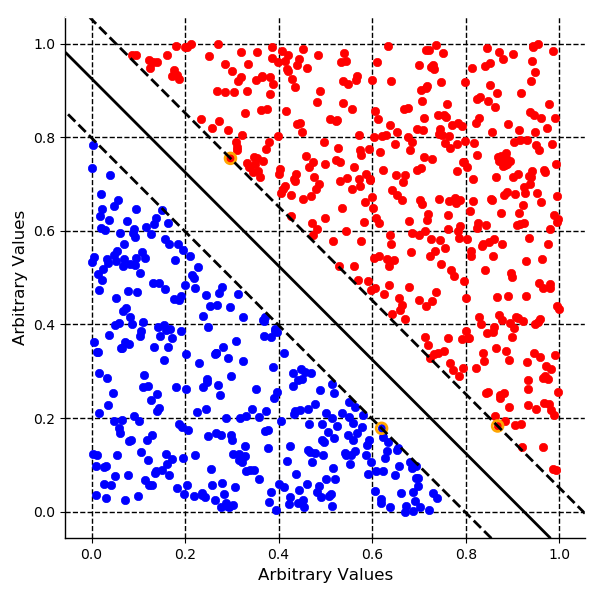
\includegraphics[width=0.5\linewidth]{Appendix1/Figs/LinSepExample.png}
 \captionof{figure}{How a support vector machine using LIBSVM trains on linear data with a separation. \hl{Axes need updating so the text is clearer}.} 
 \label{fig:LinSepExample}
\end{figure}

\begin{figure}[htbp]
 \centering
 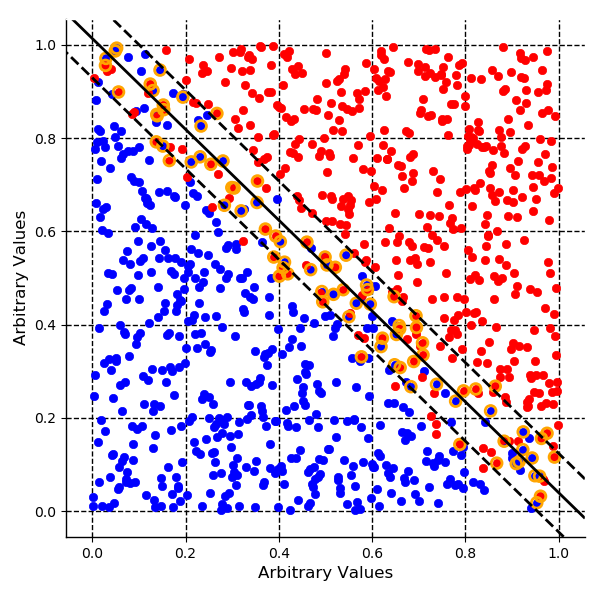
\includegraphics[width=0.5\linewidth]{Appendix1/Figs/LinNoSepExample.png}
 \captionof{figure}{How a support vector machine using LIBSVM trains on linear data with no separation. This is similar to how the neutron and noise data looks to the SVM in section \ref{sec:MachineLearningTrigger}. \hl{Axes need updating so the text is clearer}.} 
 \label{fig:LinNoSepExample}
\end{figure}

\begin{figure}[htbp]
 \centering
 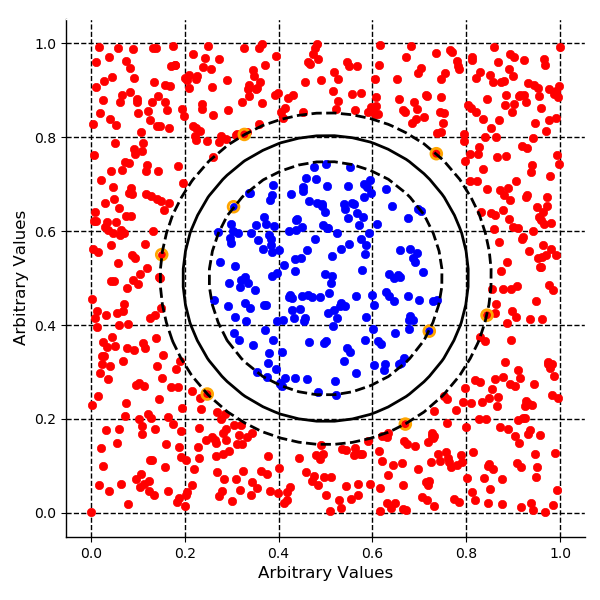
\includegraphics[width=0.5\linewidth]{Appendix1/Figs/CircleSepExample.png}
 \captionof{figure}{How the a support vector machine using LIBSVM trains on circular data with a separation. \hl{Axes need updating so the text is clearer}.} 
 \label{fig:CircleSepExample}
\end{figure}

\begin{figure}[htbp]
 \centering
 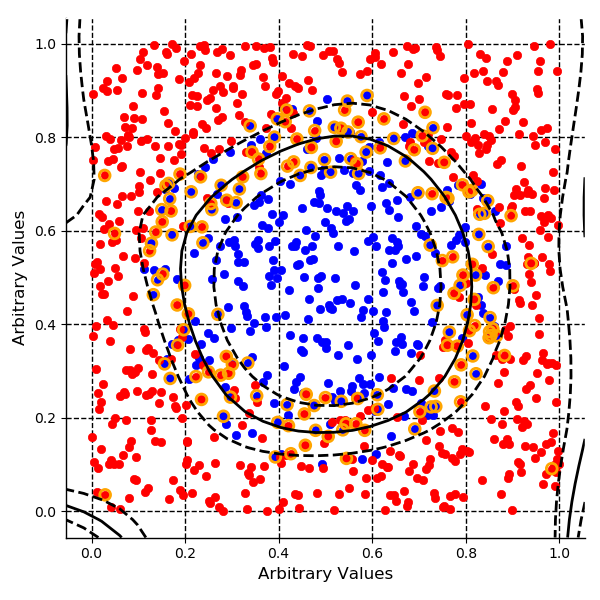
\includegraphics[width=0.5\linewidth]{Appendix1/Figs/CircleNoSepExample.png}
 \captionof{figure}{How the a support vector machine using LIBSVM trains on circular data with no separation. \hl{Axes need updating so the text is clearer}.} 
 \label{fig:CircleNoSepExample}
\end{figure}

\begin{figure}[htbp]
 \centering
 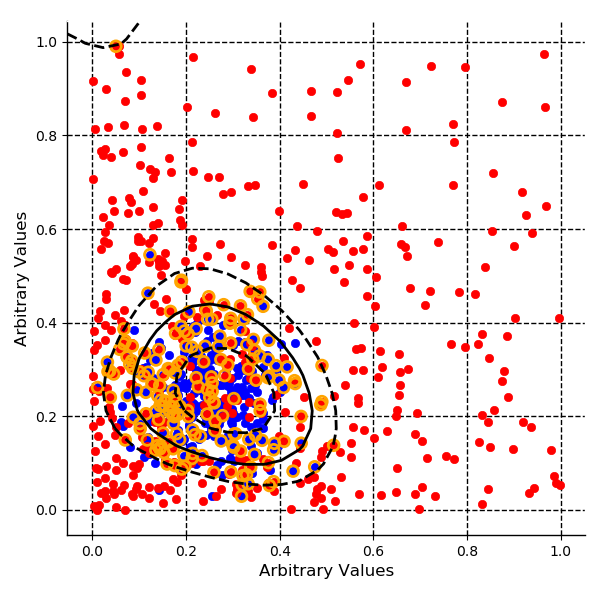
\includegraphics[width=0.5\linewidth]{Appendix1/Figs/exp_1GausseExample.png}
 \captionof{figure}{How the a support vector machine using LIBSVM trains on data with only a single Gaussian peak and exponential noise in the x and y.\hl{Axes need updating so the text is clearer}.} 
 \label{fig:exp_1GausseExample}
\end{figure}

% \section*{Windows OS}

% \subsection*{TeXLive package - full version}
% \begin{enumerate}
% \item	Download the TeXLive ISO (2.2GB) from\\
% \href{https://www.tug.org/texlive/}{https://www.tug.org/texlive/}
% \item	Download WinCDEmu (if you don't have a virtual drive) from \\
% \href{http://wincdemu.sysprogs.org/download/}
% {http://wincdemu.sysprogs.org/download/}
% \item	To install Windows CD Emulator follow the instructions at\\
% \href{http://wincdemu.sysprogs.org/tutorials/install/}
% {http://wincdemu.sysprogs.org/tutorials/install/}
% \item	Right click the iso and mount it using the WinCDEmu as shown in \\
% \href{http://wincdemu.sysprogs.org/tutorials/mount/}{
% http://wincdemu.sysprogs.org/tutorials/mount/}
% \item	Open your virtual drive and run setup.pl
% \end{enumerate}

% \begin{table}
% \caption{A nice looking table}
% \centering
% \label{table:nice_table}
% \begin{tabular}{l c c c c}
% \hline 
% \multirow{2}{*}{Dental measurement} & \multicolumn{2}{c}{Species I} & \multicolumn{2}{c}{Species II} \\ 
% \cline{2-5}
%   & mean & SD  & mean & SD  \\ 
% \hline
% I1MD & 6.23 & 0.91 & 5.2  & 0.7  \\

% I1LL & 7.48 & 0.56 & 8.7  & 0.71 \\

% I2MD & 3.99 & 0.63 & 4.22 & 0.54 \\

% I2LL & 6.81 & 0.02 & 6.66 & 0.01 \\

% CMD & 13.47 & 0.09 & 10.55 & 0.05 \\

% CBL & 11.88 & 0.05 & 13.11 & 0.04\\ 
% \hline 
% \end{tabular}
% \end{table}


% \begin{table}
% \caption{Even better looking table using booktabs}
% \centering
% \label{table:good_table}
% \begin{tabular}{l c c c c}
% \toprule
% \multirow{2}{*}{Dental measurement} & \multicolumn{2}{c}{Species I} & \multicolumn{2}{c}{Species II} \\ 
% \cmidrule{2-5}
%   & mean & SD  & mean & SD  \\ 
% \midrule
% I1MD & 6.23 & 0.91 & 5.2  & 0.7  \\

% I1LL & 7.48 & 0.56 & 8.7  & 0.71 \\

% I2MD & 3.99 & 0.63 & 4.22 & 0.54 \\

% I2LL & 6.81 & 0.02 & 6.66 & 0.01 \\

% CMD & 13.47 & 0.09 & 10.55 & 0.05 \\

% CBL & 11.88 & 0.05 & 13.11 & 0.04\\ 
% \bottomrule
% \end{tabular}
% \end{table}


